\documentclass[twoside]{book}

% Packages required by doxygen
\usepackage{fixltx2e}
\usepackage{calc}
\usepackage{doxygen}
\usepackage[export]{adjustbox} % also loads graphicx
\usepackage{graphicx}
\usepackage[utf8]{inputenc}
\usepackage{makeidx}
\usepackage{multicol}
\usepackage{multirow}
\PassOptionsToPackage{warn}{textcomp}
\usepackage{textcomp}
\usepackage[nointegrals]{wasysym}
\usepackage[table]{xcolor}

% Font selection
\usepackage[T1]{fontenc}
\usepackage[scaled=.90]{helvet}
\usepackage{courier}
\usepackage{amssymb}
\usepackage{sectsty}
\renewcommand{\familydefault}{\sfdefault}
\allsectionsfont{%
  \fontseries{bc}\selectfont%
  \color{darkgray}%
}
\renewcommand{\DoxyLabelFont}{%
  \fontseries{bc}\selectfont%
  \color{darkgray}%
}
\newcommand{\+}{\discretionary{\mbox{\scriptsize$\hookleftarrow$}}{}{}}

% Page & text layout
\usepackage{geometry}
\geometry{%
  a4paper,%
  top=2.5cm,%
  bottom=2.5cm,%
  left=2.5cm,%
  right=2.5cm%
}
\tolerance=750
\hfuzz=15pt
\hbadness=750
\setlength{\emergencystretch}{15pt}
\setlength{\parindent}{0cm}
\setlength{\parskip}{0.2cm}
\makeatletter
\renewcommand{\paragraph}{%
  \@startsection{paragraph}{4}{0ex}{-1.0ex}{1.0ex}{%
    \normalfont\normalsize\bfseries\SS@parafont%
  }%
}
\renewcommand{\subparagraph}{%
  \@startsection{subparagraph}{5}{0ex}{-1.0ex}{1.0ex}{%
    \normalfont\normalsize\bfseries\SS@subparafont%
  }%
}
\makeatother

% Headers & footers
\usepackage{fancyhdr}
\pagestyle{fancyplain}
\fancyhead[LE]{\fancyplain{}{\bfseries\thepage}}
\fancyhead[CE]{\fancyplain{}{}}
\fancyhead[RE]{\fancyplain{}{\bfseries\leftmark}}
\fancyhead[LO]{\fancyplain{}{\bfseries\rightmark}}
\fancyhead[CO]{\fancyplain{}{}}
\fancyhead[RO]{\fancyplain{}{\bfseries\thepage}}
\fancyfoot[LE]{\fancyplain{}{}}
\fancyfoot[CE]{\fancyplain{}{}}
\fancyfoot[RE]{\fancyplain{}{\bfseries\scriptsize Generated on Fri Jun 2 2017 15\+:18\+:13 for Proyecto 3 by Doxygen }}
\fancyfoot[LO]{\fancyplain{}{\bfseries\scriptsize Generated on Fri Jun 2 2017 15\+:18\+:13 for Proyecto 3 by Doxygen }}
\fancyfoot[CO]{\fancyplain{}{}}
\fancyfoot[RO]{\fancyplain{}{}}
\renewcommand{\footrulewidth}{0.4pt}
\renewcommand{\chaptermark}[1]{%
  \markboth{#1}{}%
}
\renewcommand{\sectionmark}[1]{%
  \markright{\thesection\ #1}%
}

% Indices & bibliography
\usepackage{natbib}
\usepackage[titles]{tocloft}
\setcounter{tocdepth}{3}
\setcounter{secnumdepth}{5}
\makeindex

% Hyperlinks (required, but should be loaded last)
\usepackage{ifpdf}
\ifpdf
  \usepackage[pdftex,pagebackref=true]{hyperref}
\else
  \usepackage[ps2pdf,pagebackref=true]{hyperref}
\fi
\hypersetup{%
  colorlinks=true,%
  linkcolor=blue,%
  citecolor=blue,%
  unicode%
}

% Custom commands
\newcommand{\clearemptydoublepage}{%
  \newpage{\pagestyle{empty}\cleardoublepage}%
}


%===== C O N T E N T S =====

\begin{document}

% Titlepage & ToC
\hypersetup{pageanchor=false,
             bookmarks=true,
             bookmarksnumbered=true,
             pdfencoding=unicode
            }
\pagenumbering{roman}
\begin{titlepage}
\vspace*{7cm}
\begin{center}%
{\Large Proyecto 3 }\\
\vspace*{1cm}
{\large Generated by Doxygen 1.8.9.1}\\
\vspace*{0.5cm}
{\small Fri Jun 2 2017 15:18:13}\\
\end{center}
\end{titlepage}
\clearemptydoublepage
\tableofcontents
\clearemptydoublepage
\pagenumbering{arabic}
\hypersetup{pageanchor=true}

%--- Begin generated contents ---
\chapter{R\+E\+A\+D\+M\+E}
\label{md__r_e_a_d_m_e}
\hypertarget{md__r_e_a_d_m_e}{}
Carpeta para archivos de cabecera 
\chapter{Namespace Index}
\section{Namespace List}
Here is a list of all documented namespaces with brief descriptions\+:\begin{DoxyCompactList}
\item\contentsline{section}{\hyperlink{namespaceanpi}{anpi} }{\pageref{namespaceanpi}}{}
\end{DoxyCompactList}

\chapter{Hierarchical Index}
\section{Class Hierarchy}
This inheritance list is sorted roughly, but not completely, alphabetically\+:\begin{DoxyCompactList}
\item exception\begin{DoxyCompactList}
\item \contentsline{section}{Exception}{\pageref{class_exception}}{}
\end{DoxyCompactList}
\item \contentsline{section}{anpi\+:\+:Matrix$<$ T $>$}{\pageref{classanpi_1_1_matrix}}{}
\end{DoxyCompactList}

\chapter{Class Index}
\section{Class List}
Here are the classes, structs, unions and interfaces with brief descriptions\+:\begin{DoxyCompactList}
\item\contentsline{section}{\hyperlink{class_exception}{Exception} }{\pageref{class_exception}}{}
\item\contentsline{section}{\hyperlink{classanpi_1_1_matrix}{anpi\+::\+Matrix$<$ T $>$} }{\pageref{classanpi_1_1_matrix}}{}
\end{DoxyCompactList}

\chapter{Namespace Documentation}
\hypertarget{namespaceanpi}{}\section{anpi Namespace Reference}
\label{namespaceanpi}\index{anpi@{anpi}}
\subsection*{Classes}
\begin{DoxyCompactItemize}
\item 
class \hyperlink{classanpi_1_1_matrix}{Matrix}
\end{DoxyCompactItemize}
\subsection*{Functions}
\begin{DoxyCompactItemize}
\item 
void \hyperlink{namespaceanpi_a1d6b418745abe3f2cfb4fa2dadd952f5}{liebmann} (\hyperlink{classanpi_1_1_matrix}{anpi\+::\+Matrix}$<$ double $>$ \&M, double top\+T, double right\+T, double bottom\+T, double left\+T, double lambda, double tol, bool enable\+O\+M\+P)
\item 
void \hyperlink{namespaceanpi_afabb544c6ba4b0e74c64819514dde57c}{heatflux} (\hyperlink{classanpi_1_1_matrix}{anpi\+::\+Matrix}$<$ double $>$ \&M, \hyperlink{classanpi_1_1_matrix}{anpi\+::\+Matrix}$<$ std\+::pair$<$ double, double $>$ $>$ \&M2, double top\+T, double right\+T, double bottom\+T, double left\+T, double k, bool enable\+O\+M\+P)
\item 
void \hyperlink{namespaceanpi_a4ec8112d77f2af26d8da1954cc465707}{write\+Heat\+Map} (\hyperlink{classanpi_1_1_matrix}{anpi\+::\+Matrix}$<$ double $>$ \&M, int vectorflag)
\item 
void \hyperlink{namespaceanpi_a2f885fcb56cf9214852d38588948a0d6}{write\+Flux} (\hyperlink{classanpi_1_1_matrix}{anpi\+::\+Matrix}$<$ std\+::pair$<$ double, double $>$ $>$ M)
\item 
\hypertarget{namespaceanpi_aa345df2fcc1e2936fa69be3220c3eb1d}{}{\footnotesize template$<$typename T $>$ }\\std\+::vector$<$ T $>$ {\bfseries operator$\ast$} (const std\+::vector$<$ T $>$ \&v1, const \hyperlink{classanpi_1_1_matrix}{Matrix}$<$ T $>$ \&M1)\label{namespaceanpi_aa345df2fcc1e2936fa69be3220c3eb1d}

\end{DoxyCompactItemize}
\subsection*{Variables}
\begin{DoxyCompactItemize}
\item 
\hypertarget{namespaceanpi_af2f4674639e6136c0740f304b93aca40}{}const int {\bfseries threads} = 2$\ast$omp\+\_\+get\+\_\+num\+\_\+procs()\label{namespaceanpi_af2f4674639e6136c0740f304b93aca40}

\end{DoxyCompactItemize}


\subsection{Detailed Description}


\subsection{Function Documentation}
\hypertarget{namespaceanpi_afabb544c6ba4b0e74c64819514dde57c}{}\index{anpi@{anpi}!heatflux@{heatflux}}
\index{heatflux@{heatflux}!anpi@{anpi}}
\subsubsection[{heatflux}]{\setlength{\rightskip}{0pt plus 5cm}void anpi\+::heatflux (
\begin{DoxyParamCaption}
\item[{{\bf anpi\+::\+Matrix}$<$ double $>$ \&}]{M, }
\item[{{\bf anpi\+::\+Matrix}$<$ std\+::pair$<$ double, double $>$ $>$ \&}]{M2, }
\item[{double}]{top\+T, }
\item[{double}]{right\+T, }
\item[{double}]{bottom\+T, }
\item[{double}]{left\+T, }
\item[{double}]{k, }
\item[{bool}]{enable\+O\+M\+P}
\end{DoxyParamCaption}
)}\label{namespaceanpi_afabb544c6ba4b0e74c64819514dde57c}
Esta función calcula el flujo de calor según una matriz de distribución de calor.

Parámetros\+: Matrix$<$double$>$ M matriz con la distribución de calor. \hyperlink{classanpi_1_1_matrix}{Matrix}$<$ pair$<$double,dobule$>$ $>$M2 matriz de pares de doubles donde el primer elemento es la componente \char`\"{}x\char`\"{} y el segundo es la componente \char`\"{}y\char`\"{} de cada vector de flujo, este es el resultado de la función. double top\+T temperatura que va a estar constante en la parte superior de la matriz esta no se cuenta dentro de la matriz, para aislado debe ser un Na\+N. double right\+T temperatura que va a estar constante en la parte derecha de la matriz esta no se cuenta dentro de la matriz, para aislado debe ser un Na\+N. double left\+T temperatura que va a estar constante en la parte izquierda de la matriz esta no se cuenta dentro de la matriz, para aislado debe ser un Na\+N. double bottom\+T temperatura que va a estar constante en la parte inferior de la matriz esta no se cuenta dentro de la matriz, para aislado debe ser un Na\+N. double k constante de distribución de calor del material conductor. bool enable\+O\+M\+P habilita o deshabilita la optimización de los métodos $<$ Ultima fila de la matriz

$<$ Ultima columna de la matriz \hypertarget{namespaceanpi_a1d6b418745abe3f2cfb4fa2dadd952f5}{}\index{anpi@{anpi}!liebmann@{liebmann}}
\index{liebmann@{liebmann}!anpi@{anpi}}
\subsubsection[{liebmann}]{\setlength{\rightskip}{0pt plus 5cm}void anpi\+::liebmann (
\begin{DoxyParamCaption}
\item[{{\bf anpi\+::\+Matrix}$<$ double $>$ \&}]{M, }
\item[{double}]{top\+T, }
\item[{double}]{right\+T, }
\item[{double}]{bottom\+T, }
\item[{double}]{left\+T, }
\item[{double}]{lambda, }
\item[{double}]{tol, }
\item[{bool}]{enable\+O\+M\+P}
\end{DoxyParamCaption}
)}\label{namespaceanpi_a1d6b418745abe3f2cfb4fa2dadd952f5}
Calcula la distribución de temperaturas.

Parametros\+: Matrix$<$double,double$>$ M matriz en la que se va a calcular la distribución. Se incializa en cero. double top\+T temperatura que va a estar constante en la parte superior de la matriz esta no se cuenta dentro de la matriz, para aislado debe ser un Na\+N. double right\+T temperatura que va a estar constante en la parte derecha de la matriz esta no se cuenta dentro de la matriz, para aislado debe ser un Na\+N. double left\+T temperatura que va a estar constante en la parte izquierda de la matriz esta no se cuenta dentro de la matriz, para aislado debe ser un Na\+N. double bottom\+T temperatura que va a estar constante en la parte inferior de la matriz esta no se cuenta dentro de la matriz, para aislado debe ser un Na\+N. double lambda valor para el metodo de sobre relajamiento entre 1 y 2. double tol porcentaje de error maximo que debe tener cada temperatura de la matriz bool enable\+O\+M\+P habilita o deshabilita la optimización de los métodos \hypertarget{namespaceanpi_a2f885fcb56cf9214852d38588948a0d6}{}\index{anpi@{anpi}!write\+Flux@{write\+Flux}}
\index{write\+Flux@{write\+Flux}!anpi@{anpi}}
\subsubsection[{write\+Flux}]{\setlength{\rightskip}{0pt plus 5cm}void anpi\+::write\+Flux (
\begin{DoxyParamCaption}
\item[{{\bf anpi\+::\+Matrix}$<$ std\+::pair$<$ double, double $>$ $>$}]{M}
\end{DoxyParamCaption}
)}\label{namespaceanpi_a2f885fcb56cf9214852d38588948a0d6}
Crea un archivo de extensión txt con el fin de describir la distribución de flujos de calor.

Parametros\+: Matrix$<$double$>$ M matriz que contiene las componentes de los flujos de calor de la placa \hypertarget{namespaceanpi_a4ec8112d77f2af26d8da1954cc465707}{}\index{anpi@{anpi}!write\+Heat\+Map@{write\+Heat\+Map}}
\index{write\+Heat\+Map@{write\+Heat\+Map}!anpi@{anpi}}
\subsubsection[{write\+Heat\+Map}]{\setlength{\rightskip}{0pt plus 5cm}void anpi\+::write\+Heat\+Map (
\begin{DoxyParamCaption}
\item[{{\bf anpi\+::\+Matrix}$<$ double $>$ \&}]{M, }
\item[{int}]{vectorflag}
\end{DoxyParamCaption}
)}\label{namespaceanpi_a4ec8112d77f2af26d8da1954cc465707}
Crea un archivo de extensión txt con el fin de describir la distribución de temperaturas en la placa.

Parametros\+: Matrix$<$double$>$ M matriz que contiene las temperaturas 
\chapter{Class Documentation}
\hypertarget{class_exception}{}\section{Exception Class Reference}
\label{class_exception}\index{Exception@{Exception}}


{\ttfamily \#include $<$Exception.\+hpp$>$}



Inheritance diagram for Exception\+:
\nopagebreak
\begin{figure}[H]
\begin{center}
\leavevmode
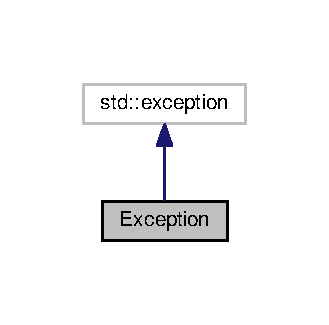
\includegraphics[width=158pt]{class_exception__inherit__graph}
\end{center}
\end{figure}


Collaboration diagram for Exception\+:
\nopagebreak
\begin{figure}[H]
\begin{center}
\leavevmode
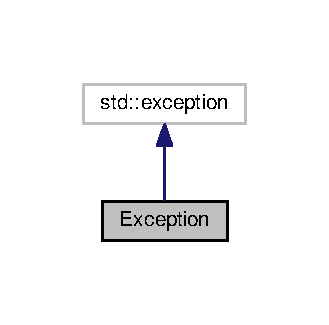
\includegraphics[width=158pt]{class_exception__coll__graph}
\end{center}
\end{figure}
\subsection*{Public Member Functions}
\begin{DoxyCompactItemize}
\item 
\hyperlink{class_exception_ac541ead5c20548813d7dea73c28c7fab}{Exception} (const char $\ast$message)
\item 
\hyperlink{class_exception_a472b7904dadf1047ba48c23741888456}{Exception} (const std\+::string \&message)
\item 
virtual \hyperlink{class_exception_ad1ba411de295ef2eeb02ba26284a829a}{$\sim$\+Exception} ()  throw ()
\item 
virtual const char $\ast$ \hyperlink{class_exception_a78154a31544a609cbd226d32574f52cd}{what} () const   throw ()
\end{DoxyCompactItemize}
\subsection*{Protected Attributes}
\begin{DoxyCompactItemize}
\item 
std\+::string \hyperlink{class_exception_a5d59cc46086c61391ed26773ce861780}{msg\+\_\+}
\end{DoxyCompactItemize}


\subsection{Detailed Description}
Excepcion general 

\subsection{Constructor \& Destructor Documentation}
\hypertarget{class_exception_ac541ead5c20548813d7dea73c28c7fab}{}\index{Exception@{Exception}!Exception@{Exception}}
\index{Exception@{Exception}!Exception@{Exception}}
\subsubsection[{Exception}]{\setlength{\rightskip}{0pt plus 5cm}Exception\+::\+Exception (
\begin{DoxyParamCaption}
\item[{const char $\ast$}]{message}
\end{DoxyParamCaption}
)\hspace{0.3cm}{\ttfamily [inline]}, {\ttfamily [explicit]}}\label{class_exception_ac541ead5c20548813d7dea73c28c7fab}
Constructor con puntero de string \hypertarget{class_exception_a472b7904dadf1047ba48c23741888456}{}\index{Exception@{Exception}!Exception@{Exception}}
\index{Exception@{Exception}!Exception@{Exception}}
\subsubsection[{Exception}]{\setlength{\rightskip}{0pt plus 5cm}Exception\+::\+Exception (
\begin{DoxyParamCaption}
\item[{const std\+::string \&}]{message}
\end{DoxyParamCaption}
)\hspace{0.3cm}{\ttfamily [inline]}, {\ttfamily [explicit]}}\label{class_exception_a472b7904dadf1047ba48c23741888456}
Constructor con objeto string \hypertarget{class_exception_ad1ba411de295ef2eeb02ba26284a829a}{}\index{Exception@{Exception}!````~Exception@{$\sim$\+Exception}}
\index{````~Exception@{$\sim$\+Exception}!Exception@{Exception}}
\subsubsection[{$\sim$\+Exception}]{\setlength{\rightskip}{0pt plus 5cm}virtual Exception\+::$\sim$\+Exception (
\begin{DoxyParamCaption}
{}
\end{DoxyParamCaption}
) throw  ) \hspace{0.3cm}{\ttfamily [inline]}, {\ttfamily [virtual]}}\label{class_exception_ad1ba411de295ef2eeb02ba26284a829a}
Destructor. 

\subsection{Member Function Documentation}
\hypertarget{class_exception_a78154a31544a609cbd226d32574f52cd}{}\index{Exception@{Exception}!what@{what}}
\index{what@{what}!Exception@{Exception}}
\subsubsection[{what}]{\setlength{\rightskip}{0pt plus 5cm}virtual const char$\ast$ Exception\+::what (
\begin{DoxyParamCaption}
{}
\end{DoxyParamCaption}
) const throw  ) \hspace{0.3cm}{\ttfamily [inline]}, {\ttfamily [virtual]}}\label{class_exception_a78154a31544a609cbd226d32574f52cd}
Retorna puntero de la descripcion de la excepcion 

\subsection{Member Data Documentation}
\hypertarget{class_exception_a5d59cc46086c61391ed26773ce861780}{}\index{Exception@{Exception}!msg\+\_\+@{msg\+\_\+}}
\index{msg\+\_\+@{msg\+\_\+}!Exception@{Exception}}
\subsubsection[{msg\+\_\+}]{\setlength{\rightskip}{0pt plus 5cm}std\+::string Exception\+::msg\+\_\+\hspace{0.3cm}{\ttfamily [protected]}}\label{class_exception_a5d59cc46086c61391ed26773ce861780}
Descricion de excepcion 

The documentation for this class was generated from the following file\+:\begin{DoxyCompactItemize}
\item 
Exception.\+hpp\end{DoxyCompactItemize}

\hypertarget{classanpi_1_1_matrix}{}\section{anpi\+:\+:Matrix$<$ T $>$ Class Template Reference}
\label{classanpi_1_1_matrix}\index{anpi\+::\+Matrix$<$ T $>$@{anpi\+::\+Matrix$<$ T $>$}}


{\ttfamily \#include $<$Matrix.\+hpp$>$}

\subsection*{Public Member Functions}
\begin{DoxyCompactItemize}
\item 
\hypertarget{classanpi_1_1_matrix_a378f41ca6eba448d5aabbbbafc9110cf}{}\hyperlink{classanpi_1_1_matrix_a378f41ca6eba448d5aabbbbafc9110cf}{Matrix} ()\label{classanpi_1_1_matrix_a378f41ca6eba448d5aabbbbafc9110cf}

\begin{DoxyCompactList}\small\item\em Construct an empty matrix. \end{DoxyCompactList}\item 
\hyperlink{classanpi_1_1_matrix_a7e948c79bd875197a3850e03efc8bd5f}{Matrix} (const size\+\_\+t \hyperlink{classanpi_1_1_matrix_a4b786272497d9f67f120a226c1bfcff4}{rows}, const size\+\_\+t \hyperlink{classanpi_1_1_matrix_a5bd9f2fe255fe0390bfe880877222b2a}{cols}, const T init\+Val=T())
\item 
\hyperlink{classanpi_1_1_matrix_a3c37c93a58cbb831863ad3ad9dc73af6}{Matrix} (const size\+\_\+t \hyperlink{classanpi_1_1_matrix_a4b786272497d9f67f120a226c1bfcff4}{rows}, const size\+\_\+t \hyperlink{classanpi_1_1_matrix_a5bd9f2fe255fe0390bfe880877222b2a}{cols}, const T $\ast$const init\+Mem)
\item 
\hyperlink{classanpi_1_1_matrix_a336997e2f4cf238db9f2fb9992144f23}{Matrix} (const \hyperlink{classanpi_1_1_matrix}{Matrix}$<$ T $>$ \&other)
\item 
\hyperlink{classanpi_1_1_matrix_acd9cb8d3e7b77bb14d9ce6d153ac5634}{$\sim$\+Matrix} ()
\item 
\hyperlink{classanpi_1_1_matrix}{Matrix}$<$ T $>$ \& \hyperlink{classanpi_1_1_matrix_acba9e336b083b5d6b58fe24f7942ddbe}{operator=} (const \hyperlink{classanpi_1_1_matrix}{Matrix}$<$ T $>$ \&other)
\item 
\hypertarget{classanpi_1_1_matrix_a6bcaaad80bd2d631017472231f6d5e63}{}T $\ast$ \hyperlink{classanpi_1_1_matrix_a6bcaaad80bd2d631017472231f6d5e63}{operator\mbox{[}$\,$\mbox{]}} (const size\+\_\+t row)\label{classanpi_1_1_matrix_a6bcaaad80bd2d631017472231f6d5e63}

\begin{DoxyCompactList}\small\item\em Return pointer to a given row. \end{DoxyCompactList}\item 
\hypertarget{classanpi_1_1_matrix_a13da6bd67304aac627c88f7213d5593c}{}const T $\ast$ \hyperlink{classanpi_1_1_matrix_a13da6bd67304aac627c88f7213d5593c}{operator\mbox{[}$\,$\mbox{]}} (const size\+\_\+t row) const \label{classanpi_1_1_matrix_a13da6bd67304aac627c88f7213d5593c}

\begin{DoxyCompactList}\small\item\em Return read-\/only pointer to a given row. \end{DoxyCompactList}\item 
\hypertarget{classanpi_1_1_matrix_aefaff4b28c12084a0c268573e96cf9ca}{}T \& \hyperlink{classanpi_1_1_matrix_aefaff4b28c12084a0c268573e96cf9ca}{operator()} (const size\+\_\+t row, const size\+\_\+t col)\label{classanpi_1_1_matrix_aefaff4b28c12084a0c268573e96cf9ca}

\begin{DoxyCompactList}\small\item\em Return reference to the element at the r row and c column. \end{DoxyCompactList}\item 
\hypertarget{classanpi_1_1_matrix_aca2952db0943940e16c715304185be7e}{}const T \& \hyperlink{classanpi_1_1_matrix_aca2952db0943940e16c715304185be7e}{operator()} (const size\+\_\+t row, const size\+\_\+t col) const \label{classanpi_1_1_matrix_aca2952db0943940e16c715304185be7e}

\begin{DoxyCompactList}\small\item\em Return const reference to the element at the r row and c column. \end{DoxyCompactList}\item 
\hyperlink{classanpi_1_1_matrix}{Matrix}$<$ T $>$ \hyperlink{classanpi_1_1_matrix_add23688fba9abe5d636abccb6ac71718}{operator+} (const \hyperlink{classanpi_1_1_matrix}{Matrix}$<$ T $>$ M1)
\item 
\hyperlink{classanpi_1_1_matrix}{Matrix}$<$ T $>$ \hyperlink{classanpi_1_1_matrix_a74bfd6dc7f3b605da2a6ea60ec90c58e}{operator-\/} (const \hyperlink{classanpi_1_1_matrix}{Matrix}$<$ T $>$ M1)
\item 
\hyperlink{classanpi_1_1_matrix}{Matrix}$<$ T $>$ \hyperlink{classanpi_1_1_matrix_aa54f3a0026abb1a06a1e8067f0094f6b}{operator$\ast$} (const \hyperlink{classanpi_1_1_matrix}{Matrix}$<$ T $>$ M1)
\item 
std\+::vector$<$ T $>$ \hyperlink{classanpi_1_1_matrix_a55ca04bf6f7275a2892b256278e25bb7}{operator$\ast$} (const std\+::vector$<$ T $>$ v1)
\item 
void \hyperlink{classanpi_1_1_matrix_ac3ac962e6058ef48b58e654e4ea7ed65}{allocate} (const size\+\_\+t row, const size\+\_\+t col)
\item 
void \hyperlink{classanpi_1_1_matrix_ad7b7f6f61d23ae8ccd7e3a19e82a8c63}{fill} (const T val)
\item 
void \hyperlink{classanpi_1_1_matrix_a2df6d413691d4aa8d0e958eb74ee394b}{fill} (const T $\ast$mem)
\item 
size\+\_\+t \hyperlink{classanpi_1_1_matrix_a4b786272497d9f67f120a226c1bfcff4}{rows} () const 
\item 
size\+\_\+t \hyperlink{classanpi_1_1_matrix_a5bd9f2fe255fe0390bfe880877222b2a}{cols} () const 
\item 
T $\ast$ \hyperlink{classanpi_1_1_matrix_ad620d822fefc019cef07f4c1fb1c7052}{data} ()
\item 
const T $\ast$ \hyperlink{classanpi_1_1_matrix_a1f1196beed4607edc1509ede6ef26217}{data} () const 
\end{DoxyCompactItemize}


\subsection{Detailed Description}
\subsubsection*{template$<$typename T$>$class anpi\+::\+Matrix$<$ T $>$}

Row-\/major simple matrix class 

\subsection{Constructor \& Destructor Documentation}
\hypertarget{classanpi_1_1_matrix_a7e948c79bd875197a3850e03efc8bd5f}{}\index{anpi\+::\+Matrix@{anpi\+::\+Matrix}!Matrix@{Matrix}}
\index{Matrix@{Matrix}!anpi\+::\+Matrix@{anpi\+::\+Matrix}}
\subsubsection[{Matrix}]{\setlength{\rightskip}{0pt plus 5cm}template$<$typename T $>$ {\bf anpi\+::\+Matrix}$<$ T $>$\+::{\bf Matrix} (
\begin{DoxyParamCaption}
\item[{const size\+\_\+t}]{rows, }
\item[{const size\+\_\+t}]{cols, }
\item[{const T}]{init\+Val = {\ttfamily T()}}
\end{DoxyParamCaption}
)}\label{classanpi_1_1_matrix_a7e948c79bd875197a3850e03efc8bd5f}
Construct a matrix rows x cols and initialize all elements with the given value \hypertarget{classanpi_1_1_matrix_a3c37c93a58cbb831863ad3ad9dc73af6}{}\index{anpi\+::\+Matrix@{anpi\+::\+Matrix}!Matrix@{Matrix}}
\index{Matrix@{Matrix}!anpi\+::\+Matrix@{anpi\+::\+Matrix}}
\subsubsection[{Matrix}]{\setlength{\rightskip}{0pt plus 5cm}template$<$typename T $>$ {\bf anpi\+::\+Matrix}$<$ T $>$\+::{\bf Matrix} (
\begin{DoxyParamCaption}
\item[{const size\+\_\+t}]{r, }
\item[{const size\+\_\+t}]{c, }
\item[{const T $\ast$const}]{init\+Mem}
\end{DoxyParamCaption}
)}\label{classanpi_1_1_matrix_a3c37c93a58cbb831863ad3ad9dc73af6}
Construct a matrix rows x cols and initialize all elements with the memory content at the given pointer \hypertarget{classanpi_1_1_matrix_a336997e2f4cf238db9f2fb9992144f23}{}\index{anpi\+::\+Matrix@{anpi\+::\+Matrix}!Matrix@{Matrix}}
\index{Matrix@{Matrix}!anpi\+::\+Matrix@{anpi\+::\+Matrix}}
\subsubsection[{Matrix}]{\setlength{\rightskip}{0pt plus 5cm}template$<$typename T $>$ {\bf anpi\+::\+Matrix}$<$ T $>$\+::{\bf Matrix} (
\begin{DoxyParamCaption}
\item[{const {\bf Matrix}$<$ T $>$ \&}]{other}
\end{DoxyParamCaption}
)}\label{classanpi_1_1_matrix_a336997e2f4cf238db9f2fb9992144f23}
Copy constructor will do a deep copy on the given matrix \hypertarget{classanpi_1_1_matrix_acd9cb8d3e7b77bb14d9ce6d153ac5634}{}\index{anpi\+::\+Matrix@{anpi\+::\+Matrix}!````~Matrix@{$\sim$\+Matrix}}
\index{````~Matrix@{$\sim$\+Matrix}!anpi\+::\+Matrix@{anpi\+::\+Matrix}}
\subsubsection[{$\sim$\+Matrix}]{\setlength{\rightskip}{0pt plus 5cm}template$<$typename T $>$ {\bf anpi\+::\+Matrix}$<$ T $>$\+::$\sim${\bf Matrix} (
\begin{DoxyParamCaption}
{}
\end{DoxyParamCaption}
)}\label{classanpi_1_1_matrix_acd9cb8d3e7b77bb14d9ce6d153ac5634}
Release all memory 

\subsection{Member Function Documentation}
\hypertarget{classanpi_1_1_matrix_ac3ac962e6058ef48b58e654e4ea7ed65}{}\index{anpi\+::\+Matrix@{anpi\+::\+Matrix}!allocate@{allocate}}
\index{allocate@{allocate}!anpi\+::\+Matrix@{anpi\+::\+Matrix}}
\subsubsection[{allocate}]{\setlength{\rightskip}{0pt plus 5cm}template$<$typename T $>$ void {\bf anpi\+::\+Matrix}$<$ T $>$\+::allocate (
\begin{DoxyParamCaption}
\item[{const size\+\_\+t}]{row, }
\item[{const size\+\_\+t}]{col}
\end{DoxyParamCaption}
)}\label{classanpi_1_1_matrix_ac3ac962e6058ef48b58e654e4ea7ed65}
Allocate memory for the given number of rows and cols \hypertarget{classanpi_1_1_matrix_a5bd9f2fe255fe0390bfe880877222b2a}{}\index{anpi\+::\+Matrix@{anpi\+::\+Matrix}!cols@{cols}}
\index{cols@{cols}!anpi\+::\+Matrix@{anpi\+::\+Matrix}}
\subsubsection[{cols}]{\setlength{\rightskip}{0pt plus 5cm}template$<$typename T$>$ size\+\_\+t {\bf anpi\+::\+Matrix}$<$ T $>$\+::cols (
\begin{DoxyParamCaption}
{}
\end{DoxyParamCaption}
) const\hspace{0.3cm}{\ttfamily [inline]}}\label{classanpi_1_1_matrix_a5bd9f2fe255fe0390bfe880877222b2a}
Number of columns \hypertarget{classanpi_1_1_matrix_ad620d822fefc019cef07f4c1fb1c7052}{}\index{anpi\+::\+Matrix@{anpi\+::\+Matrix}!data@{data}}
\index{data@{data}!anpi\+::\+Matrix@{anpi\+::\+Matrix}}
\subsubsection[{data}]{\setlength{\rightskip}{0pt plus 5cm}template$<$typename T$>$ T$\ast$ {\bf anpi\+::\+Matrix}$<$ T $>$\+::data (
\begin{DoxyParamCaption}
{}
\end{DoxyParamCaption}
)\hspace{0.3cm}{\ttfamily [inline]}}\label{classanpi_1_1_matrix_ad620d822fefc019cef07f4c1fb1c7052}
Pointer to data block \hypertarget{classanpi_1_1_matrix_a1f1196beed4607edc1509ede6ef26217}{}\index{anpi\+::\+Matrix@{anpi\+::\+Matrix}!data@{data}}
\index{data@{data}!anpi\+::\+Matrix@{anpi\+::\+Matrix}}
\subsubsection[{data}]{\setlength{\rightskip}{0pt plus 5cm}template$<$typename T$>$ const T$\ast$ {\bf anpi\+::\+Matrix}$<$ T $>$\+::data (
\begin{DoxyParamCaption}
{}
\end{DoxyParamCaption}
) const\hspace{0.3cm}{\ttfamily [inline]}}\label{classanpi_1_1_matrix_a1f1196beed4607edc1509ede6ef26217}
Pointer to data block \hypertarget{classanpi_1_1_matrix_ad7b7f6f61d23ae8ccd7e3a19e82a8c63}{}\index{anpi\+::\+Matrix@{anpi\+::\+Matrix}!fill@{fill}}
\index{fill@{fill}!anpi\+::\+Matrix@{anpi\+::\+Matrix}}
\subsubsection[{fill}]{\setlength{\rightskip}{0pt plus 5cm}template$<$typename T $>$ void {\bf anpi\+::\+Matrix}$<$ T $>$\+::fill (
\begin{DoxyParamCaption}
\item[{const T}]{val}
\end{DoxyParamCaption}
)}\label{classanpi_1_1_matrix_ad7b7f6f61d23ae8ccd7e3a19e82a8c63}
Fill all elements of the matrix with the given value \hypertarget{classanpi_1_1_matrix_a2df6d413691d4aa8d0e958eb74ee394b}{}\index{anpi\+::\+Matrix@{anpi\+::\+Matrix}!fill@{fill}}
\index{fill@{fill}!anpi\+::\+Matrix@{anpi\+::\+Matrix}}
\subsubsection[{fill}]{\setlength{\rightskip}{0pt plus 5cm}template$<$typename T $>$ void {\bf anpi\+::\+Matrix}$<$ T $>$\+::fill (
\begin{DoxyParamCaption}
\item[{const T $\ast$}]{mem}
\end{DoxyParamCaption}
)}\label{classanpi_1_1_matrix_a2df6d413691d4aa8d0e958eb74ee394b}
Fill all elements of the matrix with the given memory block

The user must ensure that the given memory block has enough elements \hypertarget{classanpi_1_1_matrix_aa54f3a0026abb1a06a1e8067f0094f6b}{}\index{anpi\+::\+Matrix@{anpi\+::\+Matrix}!operator$\ast$@{operator$\ast$}}
\index{operator$\ast$@{operator$\ast$}!anpi\+::\+Matrix@{anpi\+::\+Matrix}}
\subsubsection[{operator$\ast$}]{\setlength{\rightskip}{0pt plus 5cm}template$<$typename T$>$ {\bf Matrix}$<$T$>$ {\bf anpi\+::\+Matrix}$<$ T $>$\+::operator$\ast$ (
\begin{DoxyParamCaption}
\item[{const {\bf Matrix}$<$ T $>$}]{M1}
\end{DoxyParamCaption}
)\hspace{0.3cm}{\ttfamily [inline]}}\label{classanpi_1_1_matrix_aa54f3a0026abb1a06a1e8067f0094f6b}
Multiplicacion de matrices Algoritmo de multiplicacion de matrices \hypertarget{classanpi_1_1_matrix_a55ca04bf6f7275a2892b256278e25bb7}{}\index{anpi\+::\+Matrix@{anpi\+::\+Matrix}!operator$\ast$@{operator$\ast$}}
\index{operator$\ast$@{operator$\ast$}!anpi\+::\+Matrix@{anpi\+::\+Matrix}}
\subsubsection[{operator$\ast$}]{\setlength{\rightskip}{0pt plus 5cm}template$<$typename T$>$ std\+::vector$<$T$>$ {\bf anpi\+::\+Matrix}$<$ T $>$\+::operator$\ast$ (
\begin{DoxyParamCaption}
\item[{const std\+::vector$<$ T $>$}]{v1}
\end{DoxyParamCaption}
)\hspace{0.3cm}{\ttfamily [inline]}}\label{classanpi_1_1_matrix_a55ca04bf6f7275a2892b256278e25bb7}
Se multiplica una matriz por un vector transpuesto \hypertarget{classanpi_1_1_matrix_add23688fba9abe5d636abccb6ac71718}{}\index{anpi\+::\+Matrix@{anpi\+::\+Matrix}!operator+@{operator+}}
\index{operator+@{operator+}!anpi\+::\+Matrix@{anpi\+::\+Matrix}}
\subsubsection[{operator+}]{\setlength{\rightskip}{0pt plus 5cm}template$<$typename T$>$ {\bf Matrix}$<$T$>$ {\bf anpi\+::\+Matrix}$<$ T $>$\+::operator+ (
\begin{DoxyParamCaption}
\item[{const {\bf Matrix}$<$ T $>$}]{M1}
\end{DoxyParamCaption}
)\hspace{0.3cm}{\ttfamily [inline]}}\label{classanpi_1_1_matrix_add23688fba9abe5d636abccb6ac71718}
Sobrecarga de operador de la suma, toma cada posicion y la suma con la misma posicion de la otra matriz \hypertarget{classanpi_1_1_matrix_a74bfd6dc7f3b605da2a6ea60ec90c58e}{}\index{anpi\+::\+Matrix@{anpi\+::\+Matrix}!operator-\/@{operator-\/}}
\index{operator-\/@{operator-\/}!anpi\+::\+Matrix@{anpi\+::\+Matrix}}
\subsubsection[{operator-\/}]{\setlength{\rightskip}{0pt plus 5cm}template$<$typename T$>$ {\bf Matrix}$<$T$>$ {\bf anpi\+::\+Matrix}$<$ T $>$\+::operator-\/ (
\begin{DoxyParamCaption}
\item[{const {\bf Matrix}$<$ T $>$}]{M1}
\end{DoxyParamCaption}
)\hspace{0.3cm}{\ttfamily [inline]}}\label{classanpi_1_1_matrix_a74bfd6dc7f3b605da2a6ea60ec90c58e}
Resta las matrices, funciona de la misma manera que la suma \hypertarget{classanpi_1_1_matrix_acba9e336b083b5d6b58fe24f7942ddbe}{}\index{anpi\+::\+Matrix@{anpi\+::\+Matrix}!operator=@{operator=}}
\index{operator=@{operator=}!anpi\+::\+Matrix@{anpi\+::\+Matrix}}
\subsubsection[{operator=}]{\setlength{\rightskip}{0pt plus 5cm}template$<$typename T $>$ {\bf Matrix}$<$ T $>$ \& {\bf anpi\+::\+Matrix}$<$ T $>$\+::operator= (
\begin{DoxyParamCaption}
\item[{const {\bf Matrix}$<$ T $>$ \&}]{other}
\end{DoxyParamCaption}
)}\label{classanpi_1_1_matrix_acba9e336b083b5d6b58fe24f7942ddbe}
Deep copy another matrix \hypertarget{classanpi_1_1_matrix_a4b786272497d9f67f120a226c1bfcff4}{}\index{anpi\+::\+Matrix@{anpi\+::\+Matrix}!rows@{rows}}
\index{rows@{rows}!anpi\+::\+Matrix@{anpi\+::\+Matrix}}
\subsubsection[{rows}]{\setlength{\rightskip}{0pt plus 5cm}template$<$typename T$>$ size\+\_\+t {\bf anpi\+::\+Matrix}$<$ T $>$\+::rows (
\begin{DoxyParamCaption}
{}
\end{DoxyParamCaption}
) const\hspace{0.3cm}{\ttfamily [inline]}}\label{classanpi_1_1_matrix_a4b786272497d9f67f120a226c1bfcff4}
Number of rows 

The documentation for this class was generated from the following file\+:\begin{DoxyCompactItemize}
\item 
Matrix.\+hpp\end{DoxyCompactItemize}

%--- End generated contents ---

% Index
\backmatter
\newpage
\phantomsection
\clearemptydoublepage
\addcontentsline{toc}{chapter}{Index}
\printindex

\end{document}
